%\documentclass{article}
%\usepackage{graphicx,subfigure}
%\begin{document}

\begin{figure}[!h]
  \centering
   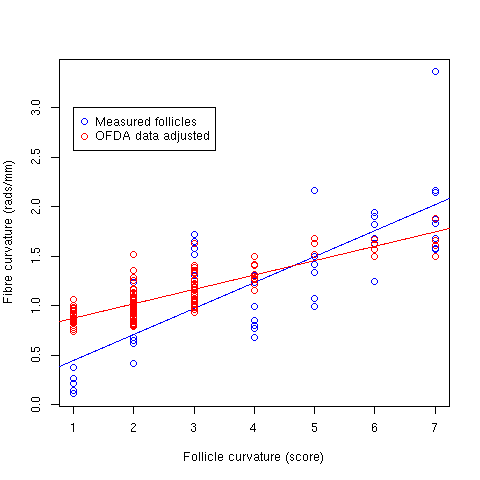
\includegraphics[width=0.9\textwidth]{ovlyint.png}
%  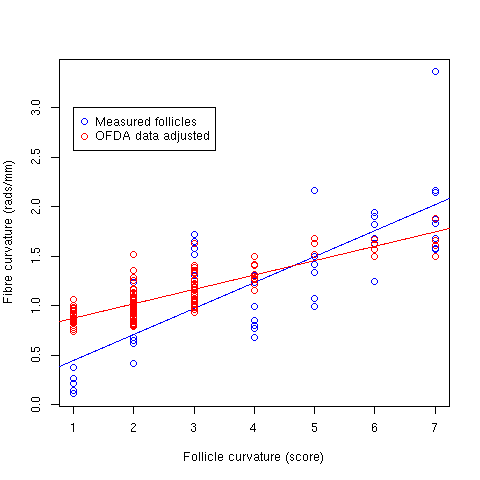
\includegraphics{ovlyint.png}
  \caption{Measured curvature of fibres in staples by OFDA technique for 159 sheep of   given follicle curvature score, superimposed on measured curvature of fibres in follicles. The OFDA mean curvture measurements for "stretched" and "unaligned" wools have been corrected to a relaxed state (intrinsic fibre curvature) assuming a stretched helix model for staple crimp. The two straight lines are orthogonal regression lines .}
  \label{fig:ovlyint}
\end{figure}

%\end{document}

